\documentclass[12pt,letterpaper]{article}
\usepackage{preamble}
\begin{document}
\title{Oil-pipeline problem}
\author{C.\ E.\ Salinas}
\date{\today}
\maketitle
\begin{abstract}
  We present a general solution to a problem from Briggs and Cochran's
  \emph{Calculus}. 
\end{abstract}

\textbf{The scenario:} A company wants to build a pipeline across a river, but
the materials required to build under the river cost $R$ dollars per mile, while
the materials required to build along the shore cost $S$ dollars per mile. Find
the least amount of money the company will have to pay in order to build a
pipeline from their location to their destination across the river.

Our first step towards a general solution to this is to label points on the
$xy$-plane accordingly, and determine the quantities which are allowed to vary.
After a moments thoughts, it is easy to see that Fig.\ \ref{fig:1} depicts the
situation accurately
\begin{figure}[htbp]
  \centering
  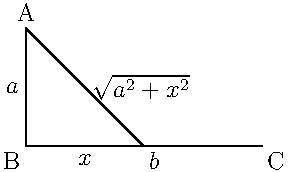
\includegraphics{figs/boat-problem}
  \caption{A picture of the general situation, with the relevant points and
    quantities labeled.}
  \label{fig:1}
\end{figure}

\end{document}
